\documentclass[12pt]{article}  % 官方要求字号不小于 12 号, 此处选择 12 号字体
 \linespread{1.1} %用来调整行距, 为标准行距的1.1倍
\usepackage{geometry} %此宏包用来调整页边距
    \geometry{left=1in,right=0.75in,top=1in,bottom=0.8in} % 搭配geometry宏包食用, 将页边距调整至特定格式.
%\usepackage{mathptmx}  % 这是 Times 字体, 中规中矩 
\usepackage{palatino}  % palatino是 COMAP 官方杂志采用的更好看的 Palatino 字体, 可替代以上的 mathptmx 宏包. 在正文中可以使用: 无衬线字体、等宽字体、斜体字体、粗体字体. 
\usepackage{pdfpages} % 可以插入一页pdf, 注意只能一页. 
\usepackage{longtable} % 可以插入跨页长表格, 同时支持冻结首行功能, 即跨页后表格第一行仍然为原表格第一行. 
\usepackage{tabu} % 更加灵活的表格制作, 可以设置列宽、行高、单元格格式, 我常用\rowfont[alignment]{fontSpec}把某行的内容置为粗体.
\usepackage{threeparttable} % 允许表格底部增加表格注释
\usepackage{listings} % 提供代码环境
\usepackage{paralist} % 提供更加方便的列表环境, 包括创建紧凑的列表、创建带有括号的行内列表
\usepackage{booktabs} % 创建更漂亮的表格, 比如经典的三线表
\usepackage{newtxtext} % 提供更多的字体
\usepackage{amsmath,amssymb,amsthm} % 经典, 没它们我会死
\usepackage{newtxmath} % must come after amsXXX
\usepackage{graphicx} % 允许插入图片、位图等. 
\usepackage{xcolor} % 允许对颜色做处理
\usepackage{fancyhdr} % 更灵活的页眉和页脚,包括自由的页码
\usepackage{float} % 为浮动体提供H命令
\usepackage{lastpage}
\usepackage{hyperref} % 允许我进行超链接
\hypersetup{colorlinks=true,urlcolor=blue}
\hypersetup{colorlinks=true,linkcolor=red}
\hypersetup{colorlinks=true,citecolor=blue}
\usepackage{subfigure} % 子图
\usepackage{multirow} % 合并列单元格

\usepackage{algorithm}% 为算法提供浮动环境
\usepackage{algorithmicx}
\usepackage{algpseudocode}

\usepackage[AutoFakeBold, AutoFakeSlant]{xeCJK}

\newtheorem{theorem}{Theorem} 
\newtheorem{corollary}{Corollary}
\newtheorem{lemma}{Lemma}
\newtheorem{definition}{Definition}
\newtheorem{proposition}{Proposition} % 呃呃太熟悉了这些

\newcommand{\blue}[1]{{\color{blue}#1}}
\renewcommand{\bf}[1]{\textbf{#1}}
% \newcommand{\bbf}[1]{{\textbf{\color{blue}#1}}}

\title{{机器学习的数学理论课程项目作业:动态Kmeans}}

\author{王英枭 \\
          211840213\\
         {\small wangbottlecap@gmail.com}}

% \bibstyle{alpha}
\bibliographystyle{alpha}

\lstset{
  language=Python,
  basicstyle=\ttfamily\small,
  numbers=left,
  numberstyle=\tiny\color{gray},
  stepnumber=1,
  numbersep=5pt,
  backgroundcolor=\color{white},
  showspaces=false,
  showstringspaces=false,
  showtabs=false,
  frame=single,
  rulecolor=\color{black},
  tabsize=2,
  captionpos=b,
  breaklines=true,
  breakatwhitespace=false,
  title=\lstname,
  keywordstyle=\color{blue},
  commentstyle=\color{green},
  stringstyle=\color{red},
  escapeinside={\%*}{*)},
  aboveskip = 10pt
  % belowskip = 10pt
}

\begin{document}

\maketitle

\begin{abstract}
本报告是25 Spring 数学学院课程《机器学习的数学理论》项目作业。针对给定的数据集,我们首先实现了经典Kmeans, Kmeans++, Hartigan \& Wong算法, Elkan加速Kmeans, miniBatch Kmeans, Bisecting Kmeans等多种算法并给出它们的主要思想和算法概述。随后,我们引入动态kmeans的概念,
考虑在动态情形下对数据进行动态聚类,并给出对应的分析。动态聚类的所有代码作为附录在报告的最后给出。
\end{abstract}
\newpage

\tableofcontents

\section{Classical Kmeans}
\subsection{问题背景与符号表示}
令数据集记为
\[
    \mathcal{X} = \{ \mathbf{x}_1, \mathbf{x}_2, \ldots, \mathbf{x}_n \} \subset \mathbb{R}^d,
\]
其中 \(\mathbf{x}_i \in \mathbb{R}^d\) 表示第 \(i\) 个样本,\(n\) 表示总样本数,\(d\) 表示特征维度。我们希望将 \(\mathcal{X}\) 划分为 \(k\) 个不相交的子集(簇)
\[
    S_1, S_2, \ldots, S_k, \quad \bigcup_{i=1}^k S_i = \mathcal{X}, \quad S_i \cap S_j = \varnothing \;(i \neq j),
\]
并为每个簇 \(S_i\) 找到一个中心 \(\boldsymbol{\mu}_i \in \mathbb{R}^d\),以最小化以下目标函数(簇内平方误差和):
\[
    J\big(S_1,\ldots,S_k; \boldsymbol{\mu}_1,\ldots,\boldsymbol{\mu}_k\big) 
    \;=\; \sum_{i=1}^k \sum_{\mathbf{x} \in S_i} \|\mathbf{x} - \boldsymbol{\mu}_i\|^2.
\]

\subsection{目标函数的分块优化思想}

KMeans 算法通过分块坐标下降(Block Coordinate Descent)策略,将优化拆分为两个交替步骤:
\begin{enumerate}
    \item 给定当前中心 \(\boldsymbol{\mu}_1,\ldots,\boldsymbol{\mu}_k\),求解最优的簇分配 \(S_1,\ldots,S_k\)。
    \item 给定当前簇分配 \(S_1,\ldots,S_k\),求解最优的聚类中心 \(\boldsymbol{\mu}_1,\ldots,\boldsymbol{\mu}_k\)。
\end{enumerate}
通过在这两个步骤间迭代更新,我们不断降低目标函数,最终在有限步内收敛到某个局部最优解。

\subsubsection{给定中心后的最优分配}
设当前中心为 \(\{\boldsymbol{\mu}_1,\ldots,\boldsymbol{\mu}_k\}\),则最优的分配策略是将每个样本分到离它最近的中心所在的簇:
\[
  \mathbf{x} \in S_i 
  \quad \Longleftrightarrow \quad
  i = \arg\min_{j \in \{1,\ldots,k\}} \|\mathbf{x} - \boldsymbol{\mu}_j\|.
\]

\subsubsection{给定分配后的最优中心}
设当前的簇分配结果为 \(S_1,\ldots,S_k\),则目标函数可表示为
\[
  J = \sum_{i=1}^k \sum_{\mathbf{x} \in S_i} \|\mathbf{x} - \boldsymbol{\mu}_i\|^2 
  \;=\; \sum_{i=1}^k J_i,
\]
其中
\(
  J_i = \sum_{\mathbf{x} \in S_i} \|\mathbf{x} - \boldsymbol{\mu}_i\|^2.
\)
要分别最小化各 \(J_i\),只需对各簇独立求解,即
\[
  \boldsymbol{\mu}_i^* = \arg\min_{\boldsymbol{\mu}_i} \sum_{\mathbf{x} \in S_i} \|\mathbf{x} - \boldsymbol{\mu}_i\|^2.
\]
可以证明此时的最优解是簇内所有样本的算术平均值:
\[
  \boldsymbol{\mu}_i^* = \frac{1}{|S_i|} \sum_{\mathbf{x} \in S_i} \mathbf{x}.
\]

\subsection{经典 KMeans 算法迭代流程}

基于上述分块最优思想,KMeans 算法流程可概括如下:
\begin{enumerate}
    \item \textbf{初始化}:随机选择 \(k\) 个样本作为初始中心,记为 \(\boldsymbol{\mu}_1^{(0)}, \ldots, \boldsymbol{\mu}_k^{(0)}\)。
    \item \textbf{迭代}:对于第 \(t\) 次迭代:
    \begin{enumerate}
        \item \emph{分配样本}(Assignment Step):
        \[
          S_i^{(t)} = \Big\{\mathbf{x} \mid 
          i = \arg\min_{j} \|\mathbf{x} - \boldsymbol{\mu}_j^{(t-1)}\| \Big\}, \quad i=1,\ldots,k.
        \]
        \item \emph{更新中心}(Update Step):
        \[
          \boldsymbol{\mu}_i^{(t)} 
          = \frac{1}{\big|S_i^{(t)}\big|} \sum_{\mathbf{x} \in S_i^{(t)}} \mathbf{x}, 
          \quad i=1,\ldots,k.
        \]
    \end{enumerate}
    \item \textbf{收敛或终止条件}:若中心更新的变化量足够小(小于某个阈值),或达到最大迭代次数,停止迭代并输出结果。
\end{enumerate}

\section{Kmeans++}
\subsection{核心思想}
与经典 KMeans 相同,令数据集
\[
  \mathcal{X} = \bigl\{ \mathbf{x}_1, \mathbf{x}_2, \ldots, \mathbf{x}_n \bigr\} \subset \mathbb{R}^d,
\]
其中 \(\mathbf{x}_i \in \mathbb{R}^d\) 表示第 \(i\) 个样本。我们希望选取 \(k\) 个“初始中心”,以改善后续 KMeans 聚类的质量和收敛速度。KMeans++ 的核心思想是:
\begin{itemize}
    \item 第一个中心等概率地从数据集中随机挑选;
    \item 后续中心依照与已选中心距离平方成正比的概率进行抽样,距离越远的点被选为新中心的概率越大。
\end{itemize}
这一策略能够让初始中心彼此分散,从而加速收敛并减少陷入不良局部最优的风险。

\subsection{初始化算法的数学步骤}
为选取第 \(k\) 个中心(假设已经选出 \(\boldsymbol{\mu}_1, \boldsymbol{\mu}_2, \ldots, \boldsymbol{\mu}_{k-1}\))时,执行以下步骤:
\begin{enumerate}
    \item \textbf{计算每个点到最近已选中心的距离平方}:  
    对每个 \(\mathbf{x}_i \in \mathcal{X}\),定义
    \[
      D(\mathbf{x}_i) 
      \;=\;
      \min_{1 \,\le\, j \,\le\, k-1}\|\mathbf{x}_i - \boldsymbol{\mu}_j\|^2.
    \]
    \item \textbf{基于距离平方构建抽样分布}:  
    \[
      P(\mathbf{x}_i)
      \;=\;
      \frac{D(\mathbf{x}_i)}{\sum_{r=1}^n D(\mathbf{x}_r)},
      \quad i = 1,2,\ldots,n.
    \]
    \item \textbf{按此分布随机抽样}:  
    随机生成一个 \(\mathbf{x}_q\) 使
    \(\Pr[q = i] = P(\mathbf{x}_i)\),并令
    \(\boldsymbol{\mu}_k = \mathbf{x}_q.\)
\end{enumerate}
当所有 \(k\) 个中心均选出后,便得到一组初始中心。

\subsection{算法描述}
\begin{algorithm}[H]
  \caption{KMeans++ Initialization}
  \begin{algorithmic}[1]
  \Require Data set $\mathcal{X} = \{\mathbf{x}_1, \ldots, \mathbf{x}_n\} \subset \mathbb{R}^d$, number of centers $k$.
  \Ensure $k$ initial centers $\boldsymbol{\mu}_1, \ldots, \boldsymbol{\mu}_k$.
  \vspace{6pt}
  \State Randomly pick one sample $\mathbf{x}_p$ from $\mathcal{X}$, set $\boldsymbol{\mu}_1 \gets \mathbf{x}_p$.
  \For{$t = 2 \to k$}
      \State \(\displaystyle \text{For each } i,\;\;D(\mathbf{x}_i) \gets 
      \min_{1 \,\le\, j \,\le\, t-1} \|\mathbf{x}_i - \boldsymbol{\mu}_j\|^2.\)
      \State \(\displaystyle P(\mathbf{x}_i) \gets 
      \frac{D(\mathbf{x}_i)}{\sum_{r=1}^n D(\mathbf{x}_r)}.\)
      \State Sample $\mathbf{x}_q$ from $\mathcal{X}$ with probability $P(\mathbf{x}_i)$.
      \State $\boldsymbol{\mu}_t \gets \mathbf{x}_q$
  \EndFor
  \State \Return $\boldsymbol{\mu}_1, \ldots, \boldsymbol{\mu}_k$
  \end{algorithmic}
  \end{algorithm}

\section{Hartigan \& Wong (1979)}
\subsection{逐点搬移的思想}
设当前数据集为
\[
  \mathcal{X} 
  \;=\; \{\mathbf{x}_1, \mathbf{x}_2, \ldots, \mathbf{x}_n\} \subset \mathbb{R}^d,
\]
被划分成 \(k\) 个簇 \(S_1, S_2, \ldots, S_k\),对应中心为
\(\boldsymbol{\mu}_1, \boldsymbol{\mu}_2, \ldots, \boldsymbol{\mu}_k\)。我们考虑将单个样本 \(\mathbf{x}\) 从其当前所在簇 \(A\) 移动到另一个簇 \(B\) 时,对目标函数
\[
  J 
  \;=\;
  \sum_{i=1}^k 
  \sum_{\mathbf{z} \in S_i}
  \|\mathbf{z} - \boldsymbol{\mu}_i\|^2
\]
所带来的变化量。具体地,令 \(S_A, S_B\) 分别表示簇 \(A\) 和簇 \(B\) 的成员集合:
\[
  S_A' = S_A \setminus \{\mathbf{x}\}, 
  \quad
  S_B' = S_B \cup \{\mathbf{x}\}.
\]
相应的新中心记为
\[
  \boldsymbol{\mu}_A' 
  = 
  \frac{1}{|S_A|-1} \sum_{\mathbf{y} \in S_A \setminus \{\mathbf{x}\}} \mathbf{y},
  \quad
  \boldsymbol{\mu}_B' 
  = 
  \frac{1}{|S_B|+1} \biggl(\sum_{\mathbf{z}\in S_B}\mathbf{z} + \mathbf{x}\biggr).
\]
若将样本 \(\mathbf{x}\) 从簇 \(A\) 搬移到簇 \(B\) 后导致目标函数值严格下降,即
\[
  \Delta 
  \;=\;
  \left(\!\sum_{\mathbf{z}\in S_A'} \|\mathbf{z} - \boldsymbol{\mu}_A'\|^2 
  + 
  \sum_{\mathbf{z}\in S_B'} \|\mathbf{z} - \boldsymbol{\mu}_B'\|^2\right)
  \;-\;
  \left(\!\sum_{\mathbf{z}\in S_A} \|\mathbf{z} - \boldsymbol{\mu}_A\|^2 
  + 
  \sum_{\mathbf{z}\in S_B} \|\mathbf{z} - \boldsymbol{\mu}_B\|^2\right)
  \;<\; 0,
\]
则执行此“逐点搬移”可使 \(J\) 单调下降,从而向局部最优解靠近。

\subsection{算法步骤}
\begin{algorithm}[H]
  \caption{Simple Hartigan \& Wong KMeans (Point Reassignment)}
  \begin{algorithmic}[1]
  \Require Data set $\mathcal{X} = \{\mathbf{x}_1, \ldots, \mathbf{x}_n\}$, number of clusters $k$, max iterations $M$.
  \Ensure Final cluster centers $\boldsymbol{\mu}_1,\ldots,\boldsymbol{\mu}_k$ and assignments $S_1,\ldots,S_k$.
  
  \vspace{6pt}
  \State Initialize centers $\boldsymbol{\mu}_1,\ldots,\boldsymbol{\mu}_k$ using some method (\textit{e.g.}, KMeans++).
  \State Assign each $\mathbf{x}_i$ to the nearest center.
  \For{$t = 1 \to M$}
      \State $\mathit{changed} \gets \text{False}$
      \For{each sample $\mathbf{x}$ in $\mathcal{X}$}
          \State Let $A$ be the cluster containing $\mathbf{x}$, and $\boldsymbol{\mu}_A$ be its center.
          \State $\delta_{\text{best}} \gets 0,\quad B_{\text{best}} \gets A$
          \For{each cluster $B \neq A$}
              \State Compute the new centers if $\mathbf{x}$ were moved from $A$ to $B$:
              \[
                \boldsymbol{\mu}_A' \quad \text{and} \quad \boldsymbol{\mu}_B'.
              \]
              \State Evaluate $\Delta = J_{\text{after}} - J_{\text{before}}$ for the local change (see text).
              \If{$\Delta < \delta_{\text{best}}$}
                  \State $\delta_{\text{best}} \gets \Delta$
                  \State $B_{\text{best}} \gets B$
              \EndIf
          \EndFor
          \If{$B_{\text{best}} \neq A$}
              \State Move $\mathbf{x}$ from $A$ to $B_{\text{best}}$, update $\boldsymbol{\mu}_A$ and $\boldsymbol{\mu}_{B_{\text{best}}}$.
              \State $\mathit{changed} \gets \text{True}$
          \EndIf
      \EndFor
      \If{not $\mathit{changed}$}
          \State \textbf{break}
      \EndIf
  \EndFor
  \State \textbf{return} final centers $\{\boldsymbol{\mu}_1,\ldots,\boldsymbol{\mu}_k\}$ and cluster sets $\{S_1,\ldots,S_k\}$.
  \end{algorithmic}
  \end{algorithm}

\section{Elkan 加速版}

\subsection{主要思想}
与经典 KMeans 相同,假设数据集为
\[
  \mathcal{X} 
  = \{\mathbf{x}_1, \mathbf{x}_2, \dots, \mathbf{x}_n\} 
  \subset \mathbb{R}^d,
\]
聚类中心为 
\(\boldsymbol{c}_1, \boldsymbol{c}_2, \ldots, \boldsymbol{c}_k\),
目标函数为
\[
  J 
  = \sum_{i=1}^k 
  \sum_{\mathbf{x} \in S_i}
  \|\mathbf{x} - \boldsymbol{c}_i\|^2.
\]
Elkan 加速版的关键在于利用对偶边界(上下界)和三角不等式减少不必要的距离计算。大体上,为每个样本 $\mathbf{x}$ 维护:

\begin{itemize}
    \item \textbf{上界} $u(\mathbf{x})$:估计 $\mathbf{x}$ 与其当前分配中心 $\boldsymbol{c}_{\mathrm{assigned}(\mathbf{x})}$ 的距离,
    \[
      u(\mathbf{x}) 
      \;\ge\; 
      \|\mathbf{x} - \boldsymbol{c}_{\mathrm{assigned}(\mathbf{x})}\|.
    \]
    \item \textbf{下界} $l_j(\mathbf{x})$:对任意中心 $\boldsymbol{c}_j$ 的距离,
    \[
      l_j(\mathbf{x}) 
      \;\le\; 
      \|\mathbf{x} - \boldsymbol{c}_j\|.
    \]
\end{itemize}

记中心间的距离为
\[
  d_{ij} 
  = \|\boldsymbol{c}_i - \boldsymbol{c}_j\|.
\]
若对样本 $\mathbf{x}$ 有
\[
  u(\mathbf{x}) 
  < 
  \frac{d_{ij}}{2},
\]
则可推断
\(\|\mathbf{x} - \boldsymbol{c}_j\| 
> 
\|\mathbf{x} - \boldsymbol{c}_i\|\),
因此中心 $j$ 不会是 $\mathbf{x}$ 更好的分配对象,无需计算真实距离。三角不等式保障了此结论的正确性,从而实现大规模剪枝。  
此外,当中心 $\boldsymbol{c}_i$ 在两次迭代间移动量 $m_i$ 较小,则可依据
\[
  u(\mathbf{x}) 
  \leftarrow 
  u(\mathbf{x}) + m_i
\]
等方式修正上界,而依旧保留安全的剪枝判断。此即 Elkan 加速算法的根本逻辑:\textbf{以有限的上/下界更新与三角不等式将大量“无关距离”排除在外},从而减少时间复杂度。

\subsection{算法框架}
\begin{algorithm}[H]
  \caption{Elkan Accelerated KMeans}
  \begin{algorithmic}[1]
  \Require Data set $\mathcal{X} = \{\mathbf{x}_1,\dots,\mathbf{x}_n\}$, number of clusters $k$, max iterations $M$.
  \Ensure Cluster centers $\{\boldsymbol{c}_1,\dots,\boldsymbol{c}_k\}$ and partition $S_1,\dots,S_k$.
  
  \vspace{6pt}
  \State Initialize centers $\boldsymbol{c}_1,\dots,\boldsymbol{c}_k$ (e.g., KMeans++), and assign each sample to the nearest center.
  \State For each $\mathbf{x}_i$, set $u(\mathbf{x}_i) \gets \|\mathbf{x}_i - \boldsymbol{c}_{\mathrm{assigned}(\mathbf{x}_i)}\|$, and initialize $l_j(\mathbf{x}_i)$ for $j \neq \mathrm{assigned}(\mathbf{x}_i)$.
  \For{$t=1 \to M$}
      \State \textbf{Update bounds:} compute center movements $m_i = \|\boldsymbol{c}_i^{(\text{old})}-\boldsymbol{c}_i^{(\text{new})}\|$ and correct $u(\mathbf{x})$ or $l_j(\mathbf{x})$ accordingly.
      \State \textbf{Assignment step:}
          \For{each sample $\mathbf{x}_i$}
              \State Let $i_0 = \mathrm{assigned}(\mathbf{x}_i)$.
              \For{each center $j \neq i_0$}
                  \State \textbf{Pruning check}: if $u(\mathbf{x}_i) < d_{i_0 j} / 2$, skip distance computation for center $j$.
                  \State Otherwise, compute $\|\mathbf{x}_i - \boldsymbol{c}_j\|$ and update $u(\mathbf{x}_i), l_j(\mathbf{x}_i)$ if needed.
              \EndFor
              \State Re-assign $\mathbf{x}_i$ to the closest center found if it differs from $i_0$.
          \EndFor
      \State \textbf{Update step:} recalculate each center $\boldsymbol{c}_j \gets \frac{1}{|S_j|}\sum_{\mathbf{x}\in S_j}\mathbf{x}$.
      \State \textbf{Check convergence:} if center changes are small enough or no re-assignments, break.
  \EndFor
  \State \textbf{return} $\{\boldsymbol{c}_1,\dots,\boldsymbol{c}_k\}$ and final partition $\{S_1,\dots,S_k\}$.
  \end{algorithmic}
  \end{algorithm}

\section{Mini-Batch KMeans}

\subsection{主要思想}
与经典 KMeans 相同,假设数据集
\[
  \mathcal{X} \;=\; \{\mathbf{x}_1,\mathbf{x}_2,\dots,\mathbf{x}_n\} \,\subset \,\mathbb{R}^d,
\]
我们希望寻找 $k$ 个中心 $\boldsymbol{\mu}_1,\dots,\boldsymbol{\mu}_k$ 并将 $\mathcal{X}$ 划分为 $k$ 个不相交子集 $S_1,\dots,S_k$,使得以下目标函数(簇内平方误差和)最小化:
\[
  \min_{S_1,\dots,S_k;\;\boldsymbol{\mu}_1,\dots,\boldsymbol{\mu}_k}
  \;\;
  \sum_{j=1}^k 
  \sum_{\mathbf{x}\in S_j}
  \|\mathbf{x} - \boldsymbol{\mu}_j\|^2.
\]
然而,在大规模数据场景或流式数据场景中,每次迭代都处理全部样本 $\{\mathbf{x}_1,\dots,\mathbf{x}_n\}$ 成本非常高。为此,Mini-Batch KMeans 在每次迭代只抽取一个 \textbf{小批量}(mini-batch),记为
\[
  B^{(t)} \;=\; \{\mathbf{x}_{i_1}, \dots, \mathbf{x}_{i_m}\} \,\subset \,\mathcal{X}, 
  \quad |B^{(t)}| = m \ll n,
\]
并执行类似 KMeans 的分配与更新步骤,但仅基于 $B^{(t)}$ 更新当前的中心 $\{\boldsymbol{\mu}_j\}$。

令在 $B^{(t)}$ 中分配到簇 $j$ 的那些样本记为
\[
  B^{(t)}_j 
  \;=\; 
  \bigl\{\mathbf{x} \in B^{(t)} \mid \text{assigned to } \boldsymbol{\mu}_j\bigr\},
\]
则 $\boldsymbol{\mu}_j$ 的更新常采取如下形式:
\[
  \boldsymbol{\mu}_j^{(t+1)} 
  \;=\;
  \boldsymbol{\mu}_j^{(t)} 
  \;+\; \eta 
  \left(
    \overline{\mathbf{x}}_{\text{batch},\,j} 
    \;-\;
    \boldsymbol{\mu}_j^{(t)}
  \right),
\]
其中
\[
  \overline{\mathbf{x}}_{\text{batch},\,j}
  \;=\;
  \frac{1}{\bigl|B_j^{(t)}\bigr|}
  \sum_{\mathbf{x} \in B_j^{(t)}} 
  \mathbf{x}, 
\quad
  \eta \in (0,1]
\]
为更新步长(又可视为学习率)。这使得中心向本批次样本的均值方向移动,而无需处理全部 $n$ 个样本。

通过在每次迭代使用较小规模的批数据 $B^{(t)}$,算法单次迭代的复杂度降至 $O(mk)$,明显低于经典 KMeans 的 $O(nk)$;同时在多轮迭代后,聚类解可近似逼近全量 KMeans 的结果。Mini-Batch KMeans 在大规模数据或在线学习环境中非常实用,能在保证一定精度下显著降低计算开销。

\subsection{算法框架}
\begin{algorithm}[H]
  \caption{Mini-Batch KMeans}
  \begin{algorithmic}[1]
    \Require Data set $\mathcal{X} = \{\mathbf{x}_1,\dots,\mathbf{x}_n\}\subset \mathbb{R}^d$, 
      number of clusters $k$, mini-batch size $m$, max iterations $M$.
    \Ensure Final centers $\{\boldsymbol{\mu}_1,\dots,\boldsymbol{\mu}_k\}$ and assignments $S_1,\dots,S_k$.

    \vspace{6pt}
    \State Initialize centers $\boldsymbol{\mu}_1,\dots,\boldsymbol{\mu}_k$ (e.g., random or KMeans++).
    \For{$t = 1 \to M$}
      \State \textbf{Sample a mini-batch} $B^{(t)} = \{\mathbf{x}_{i_1},\dots,\mathbf{x}_{i_m}\} \subset \mathcal{X}$.
      \State \textbf{Assignment step (on mini-batch)}:
        \For{each $\mathbf{x} \in B^{(t)}$}
            \State Find $j^* = \arg\min_{j} \|\mathbf{x} - \boldsymbol{\mu}_j\|^2$.
            \State Assign $\mathbf{x}$ to cluster $j^*$.
        \EndFor
      \State \textbf{Update step (on mini-batch)}:
        \For{$j = 1 \to k$}
          \State Let $B_j^{(t)}$ be the subset of $B^{(t)}$ assigned to center $j$.
          \If{$B_j^{(t)} \neq \varnothing$}
            \State $\overline{\mathbf{x}}_{j}^{(t)} \gets \frac{1}{|B_j^{(t)}|} \sum_{\mathbf{x}\in B_j^{(t)}} \mathbf{x}$.
            \State $\boldsymbol{\mu}_j \gets \boldsymbol{\mu}_j + \eta\left(\overline{\mathbf{x}}_{j}^{(t)} - \boldsymbol{\mu}_j\right)$,
            \State \quad \textit{where $\eta$ is a learning rate in $(0,1]$.}
          \EndIf
        \EndFor
      \State \textbf{(Optional) Check convergence} if center movement is small or no changes.
    \EndFor

    \State \textbf{Final assignment}: reassign every $\mathbf{x}_i\in \mathcal{X}$ to its nearest center $\boldsymbol{\mu}_j$.
    \State \textbf{return} $\{\boldsymbol{\mu}_1,\dots,\boldsymbol{\mu}_k\}$ and $S_1,\dots,S_k$.
  \end{algorithmic}
\end{algorithm}

\section{Bisecting KMeans}

\subsection{主要思想}
Bisecting KMeans(又称二分 KMeans)将 KMeans 与层次聚类思想结合,通过 \textbf{自顶向下} (top-down) 的分裂方式得到 $k$ 个簇。初始时将所有数据视为一个大簇,然后反复挑选其中“最需要细分”的簇,做 2-means 将其分成两个簇,直至达到 $k$ 个簇。

具体而言,令 $\mathcal{X}$ 初始在一个簇 $S_{\text{root}} = \{\mathbf{x}_1,\dots,\mathbf{x}_n\}$ 中,中心
\[
  \boldsymbol{\mu}_{\text{root}}
  \;=\;
  \frac{1}{n}
  \sum_{i=1}^n \mathbf{x}_i.
\]
若当前聚类数小于 $k$,则:
\begin{enumerate}
\item 选出一个簇 $S_{\max}$(可根据簇内误差最大的原则),其中包含若干样本 $\{\mathbf{x}_{\alpha_1}, \dots, \mathbf{x}_{\alpha_r}\}$。
\item 在该簇上运行 \textbf{2-means}($k=2$ 的 KMeans),解为
\[
  \min_{S_a,\,S_b,\;\boldsymbol{\mu}_a,\,\boldsymbol{\mu}_b}
  \left(
    \sum_{\mathbf{x}\in S_a}\|\mathbf{x} - \boldsymbol{\mu}_a\|^2
    \;+\;
    \sum_{\mathbf{x}\in S_b}\|\mathbf{x} - \boldsymbol{\mu}_b\|^2
  \right),
\]
使 $S_a \cup S_b = S_{\max},\, S_a \cap S_b = \varnothing$。
\item 用 $S_a$ 与 $S_b$ 替换 $S_{\max}$,整体簇数加 1。
\end{enumerate}

通过这种不断“二分”最大的簇,Bisecting KMeans 最终可得到 $k$ 个簇。其核心思想是:
\[
  \text{逐次选出最需要被拆分的簇,用 } 2\text{-means 精细地对它进行划分。}
\]
在每次二分时,仍遵循 KMeans 的优化目标,即最小化簇内误差和,只不过将问题限制在某个子簇 $S_{\max}$ 上。这种自顶向下的层次聚类与 KMeans 结合的方式在实践中具有较好的可解释性和灵活度,同时每次只在局部簇做细分,能在一定程度上减少计算量。虽然与一次性 $k$-means 一样只能得到局部最优,但常能更好地针对层次结构做可视化与分析。


\subsection{算法框架}
\begin{algorithm}[H]
  \caption{Bisecting KMeans (二分聚类)}
  \begin{algorithmic}[1]
    \Require Data set $\mathcal{X} = \{\mathbf{x}_1,\dots,\mathbf{x}_n\}\subset \mathbb{R}^d$, number of clusters $k$, max iterations for each 2-means $M_2$.
    \Ensure $k$ final clusters $S_1,\dots,S_k$ with centers $\{\boldsymbol{\mu}_1,\dots,\boldsymbol{\mu}_k\}$.

    \vspace{6pt}
    \State Initialize a single cluster $S_{\text{root}} = \{\mathbf{x}_1,\dots,\mathbf{x}_n\}$.
    \State Let the set of active clusters $\mathcal{C} \gets \{S_{\text{root}}\}$.
    \While{$|\mathcal{C}| < k$}
      \State Select the cluster $S_{\max} \in \mathcal{C}$ with the largest SSE (or largest cardinality).
      \State Remove $S_{\max}$ from $\mathcal{C}$.

      \State \textbf{Run 2-means} on $S_{\max}$ (e.g., use Lloyd or Mini-Batch with $k=2$, $M_2$ iterations):
        \State \quad Split $S_{\max}$ into two subsets $S_a$ and $S_b$ with centers $\boldsymbol{\mu}_a$ and $\boldsymbol{\mu}_b$.

      \State Add $S_a$ and $S_b$ to $\mathcal{C}$.

    \EndWhile

    \State Let $\{S_1,\dots,S_k\} = \mathcal{C}$, and compute each center as $\boldsymbol{\mu}_j \gets \frac{1}{|S_j|}\sum_{\mathbf{x}\in S_j}\mathbf{x}$.
    \State \textbf{return} $S_1,\dots,S_k$ and $\{\boldsymbol{\mu}_1,\dots,\boldsymbol{\mu}_k\}$.
  \end{algorithmic}
\end{algorithm}


\section{动态聚类}
\subsection{问题描述}
随着海量数据以流式方式到达,本节所述算法旨在对数据进行动态聚类。假设数据流被划分为等长批次,每批含 $B=100$ 条样本。记在时刻 $t$ 到达的新批次为 $\Delta\mathcal{D}_t$,总体数据集为
\[
\mathcal{D}_t=\bigcup_{s=1}^t\Delta\mathcal{D}_s.
\]
我们要求:
\begin{itemize}
  \item 每批到达后立即更新聚类结构;
  \item 保证每个簇包含的数据条数在 $[N_{\min},N_{\max}]=[60,150]$ 范围内;
  \item 若某簇大小超过 $N_{\max}$,则将其拆分为两个子簇;
  \item (可扩展)若删除过期数据后某簇小于 $N_{\min}$,则与最近邻簇合并。
\end{itemize}

\subsection{数学建模}
令第 $t$ 时刻的聚类中心集合为
\[
C_t=\{\,c_{t,1},\dots,c_{t,K_t}\},\quad c_{t,i}\in\mathbb{R}^d,
\]
样本点集合被分配至簇 $\mathcal{D}_{t,i}=\{\,x\mid \mathrm{assign}(x)=i\}$。我们仍以 KMeans 惯性(Inertia)作为损失函数:
\[
\mathcal{L}_t \;=\;\sum_{i=1}^{K_t}\sum_{x\in\mathcal{D}_{t,i}}\|x - c_{t,i}\|^2.
\]
动态更新包含以下运算:
\begin{enumerate}
  \item \textbf{增量指派}:对新到达点 $x\in\Delta\mathcal{D}_t$,
  \[
    \mathrm{assign}(x)
    =\arg\min_{1\le i\le K_{t-1}}\|x - c_{t-1,i}\|.
  \]
  \item \textbf{中心更新}:重新计算
  \[
    c_{t,i}
    =\frac{1}{|\mathcal{D}_{t,i}|}\sum_{x\in\mathcal{D}_{t,i}} x.
  \]
  \item \textbf{簇拆分}:对所有 $i$ 满足 $|\mathcal{D}_{t,i}|>N_{\max}$,
  在该簇内部再执行一次 $k=2$ 的 KMeans,得子中心 $\{c'_{i,1},c'_{i,2}\}$,
  用 $c'_{i,1}$ 替换原中心并新增 $c'_{i,2}$。
\end{enumerate}

\subsection{算法流程}
\begin{algorithm}[h]
  \caption{Dynamic KMeans Clustering Algorithm}
  \label{alg:dynamic_kmeans}
  \begin{algorithmic}[1]
    \Require Data stream $\{\Delta\mathcal{D}_t\}_{t=1}^T$, batch size $B$, thresholds $N_{\min},N_{\max}$
    \Ensure Final cluster centers $C_T$
    \State $t \gets 1$
    \State Perform standard KMeans on $\Delta\mathcal{D}_1$ to obtain $C_1,\;A_1$
    \For{$t = 2,3,\dots,T$}
      \State Read new batch $\Delta\mathcal{D}_t$
      \ForAll{$x\in \Delta\mathcal{D}_t$}
        \State $\mathrm{assign}(x)\gets\arg\min_{i}\|x - c_{t-1,i}\|$
      \EndFor
      \State Update centers: $c_{t,i}\gets\frac{1}{|\mathcal{D}_{t,i}|}\sum_{x\in\mathcal{D}_{t,i}}x$
      \ForAll{clusters $i$ with $|\mathcal{D}_{t,i}|>N_{\max}$}
        \State Run 2-cluster KMeans on $\mathcal{D}_{t,i}$ to get $\{c'_{i,1},c'_{i,2}\}$
        \State Replace $c_{t,i}\gets c'_{i,1}$ and add new center $c'_{i,2}$
      \EndFor
    \EndFor
  \end{algorithmic}
\end{algorithm}

\subsection{复杂度分析}
该算法包含三个主要步骤:增量指派、中心更新、簇拆分,现逐一给出详细复杂度推导。

\subsubsection{增量指派 Complexity of Assignment}
在第 $t$ 批处理中,新数据量为 $B$,当前簇数为 $K_{t-1}$,数据维度为 $d$。对每个点计算到 $K_{t-1}$ 个中心的欧氏距离,时间复杂度为
\[
O\left(B \times K_{t-1} \times d\right).
\]
由于 $K_{t-1}$ 保持在总数据条数 $n_t$ 的 1\% 左右,即 $K_{t-1}\approx 0.01\,n_t/B$,故该步骤总体接近线性。

\subsubsection{中心更新 Complexity of Update}
中心更新需遍历所有簇及其成员,总数据量为 $n_t=\sum_i|\mathcal{D}_{t,i}|$,对每簇计算均值耗时 $O(|\mathcal{D}_{t,i}|\times d)$,合计
\[
\sum_{i=1}^{K_t}O\left(|\mathcal{D}_{t,i}|\times d\right)
=O\left(n_t\times d\right).
\]

\subsubsection{簇拆分 Complexity of Split}
最坏情况下,每个簇都可能超过阈值并被拆分,拆分过程对簇内点再执行一次 $k=2$ KMeans。对簇 $i$,若其规模为 $m_i$,一次 2-簇 KMeans 时间为 $O(m_i\times d)$(假设迭代次数有限常数次)。合并所有簇的拆分成本为
\[
\sum_{i=1}^{K_t}O\left(m_i\times d\right)
=O\left(n_t\times d\right).
\]

\subsection{整体复杂度 Overall Complexity}
综合上述三步,每批次迭代的总复杂度为
\[
O\left(BK_{t-1}d + n_t d + n_t d\right)
=O\left((B K_{t-1} + 2 n_t)\,d\right).
\]
鉴于 $B\ll n_t$ 且 $K_{t-1}=O(n_t/B)$,可简化为
\[
O\left(n_t\,d\right),
\]
即对流式数据的聚类更新具有近线性时间复杂度,适用于大规模在线场景。


\section{程序结果}
在给定迭代步数和给定收敛时间的收敛曲线中,Minibatch和Bisecting聚类算法都比经典kmeans有了明显的提速。同时,由于算法自身设计,Bisecting的聚类速度相对更稳定,MiniBatch算法更加依赖挑选Batch的策略。
\begin{figure}[H]
  \centering
  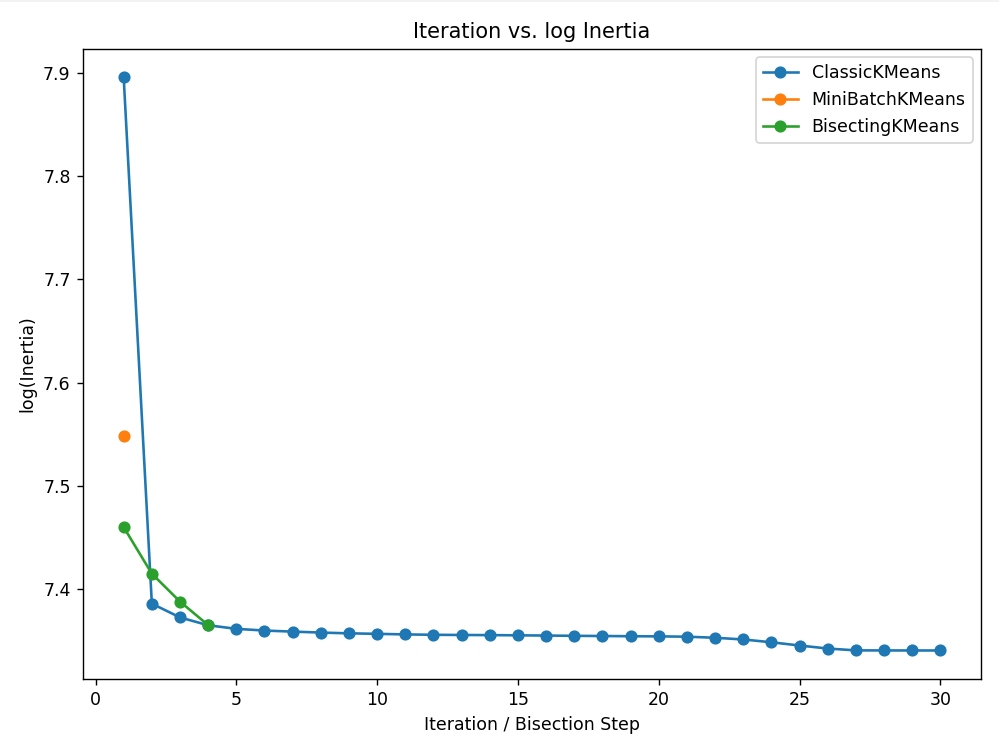
\includegraphics[width=0.7\textwidth]{kmeansII_IterVSlogLoss.png} % 图片路径
  \caption{IterVSlogLoss}
\end{figure}

\begin{figure}[H]
  \centering
  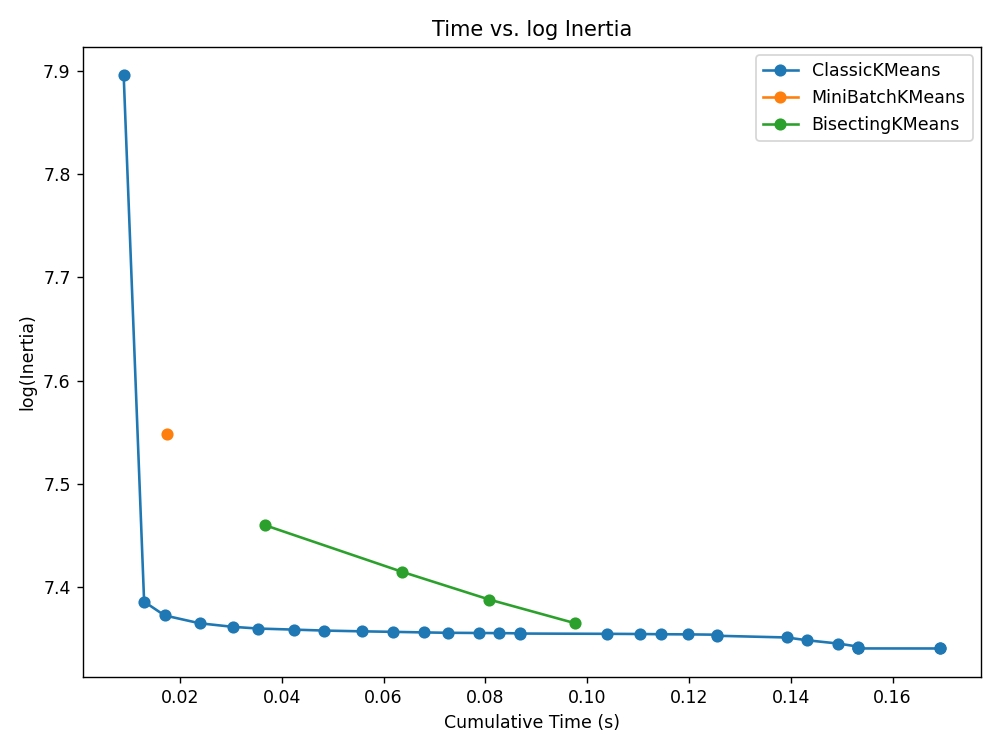
\includegraphics[width=0.7\textwidth]{kmeansII_TimeVSlogLoss.png} % 图片路径
  \caption{TimeVSlogLoss}
\end{figure}


聚类效果如下:
\begin{figure}[htbp]
  \centering
  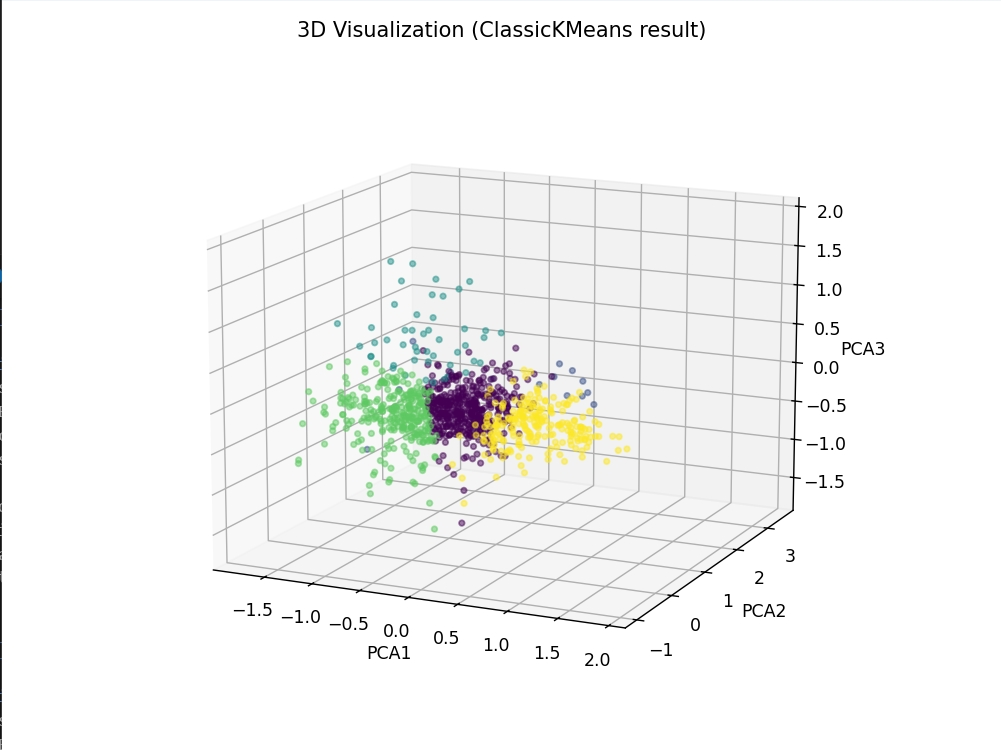
\includegraphics[width=0.7\textwidth]{kmeansII_PCA.png} % 图片路径
  \caption{TimeVSlogLoss}
\end{figure}

随后,针对动态聚类问题,我们计算得出在相同的中心数量下,动态方法和静态方法平均最近距离为0.3699。随着引入数据的增大,
动态方法的Loss函数也在递增,这种递增方式无法避免,因而需要更加具有代表性的loss函数设计以表达在动态过程中聚类的效果;
时间方面,动态方法引入时间较长,这一方面是因为动态方法需要多次调用kmeans和裂分裂函数,另外一方面是因为动态方法也会对
原始数据进行重复读取。当使用数据量较大(如百万条以上)时,动态方法因其快速迭代初始解和分批读取数据对内存需求较低等特性
会相较本次实验出现不同的表现。



\begin{figure}[htbp]
  \centering
  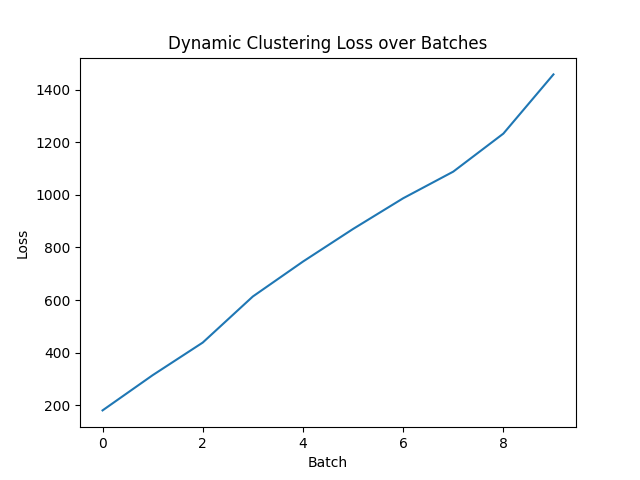
\includegraphics[width=0.7\textwidth]{dynLoss.png} % 图片路径
  \caption{Dynamic Method: Loss}
\end{figure}

\begin{figure}[htbp]
  \centering
  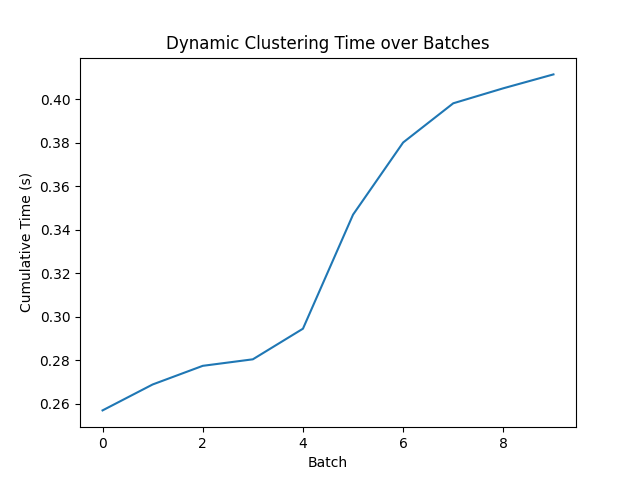
\includegraphics[width=0.7\textwidth]{dynTime.png} % 图片路径
  \caption{Dynamic Method: Time}
\end{figure}

\begin{figure}[htbp]
  \centering
  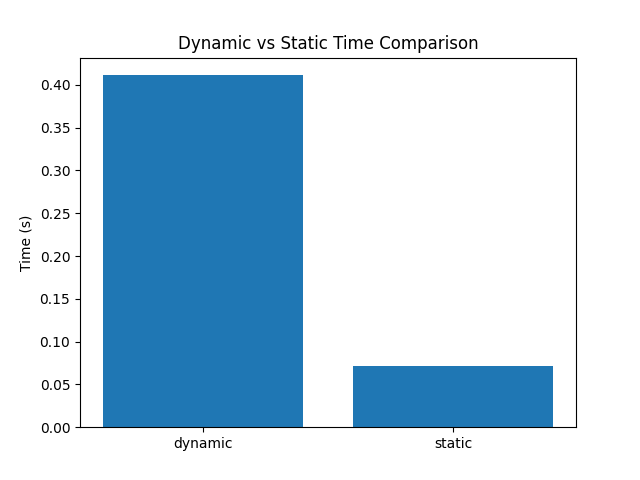
\includegraphics[width=0.7\textwidth]{TimeCompare.png} % 图片路径
  \caption{Time Compare}
\end{figure}

\end{document}